\documentclass[11pt]{article}

\usepackage[margin=1in]{geometry}
\usepackage[T1]{fontenc}
\usepackage[utf8]{inputenc}
\usepackage{lmodern}
\usepackage{microtype}
\usepackage{amsmath}
\usepackage{amssymb}
\usepackage{array}
\usepackage{booktabs}
\usepackage{graphicx}
\usepackage{subcaption}
\usepackage{float}
\usepackage{xcolor}
\usepackage{siunitx}
\usepackage{orcidlink}
\usepackage{hyperref}
\usepackage[nameinlink,noabbrev]{cleveref}

\graphicspath{{figures/}}

\hypersetup{
  colorlinks=true,
  linkcolor=blue,
  citecolor=blue,
  urlcolor=blue
}

\sisetup{
  detect-all,
  separate-uncertainty=true
}

% V2 review highlighting; supports page breaks.
\usepackage{mdframed}

\newcommand{\dft}{\mathrm{DFT}}
\newcommand{\xtb}{\mathrm{xTB}}
\newcommand{\boe}{\mathrm{BoE}}
\newcommand{\pre}{\mathrm{PRE}}
\newcommand{\gemnet}{\mathrm{GemNet}}
\newcommand{\qmNine}{\mathrm{QM9}}
\newcommand{\tmqm}{\mathrm{tmQM}}
\newcommand{\target}{y}
\newcommand{\baseline}{b}
\newcommand{\residual}{r}
\newcommand{\prediction}{\hat{y}}
\newcommand{\mae}{\mathrm{MAE}}
\newcommand{\rTwo}{R^2}


\title{Beyond Variance Reduction: Target Design for Generalizable Machine-Learning Interatomic Potentials}
\author{
  \orcidlink{0000-0002-1168-9830}\hspace{1mm}Kareem M.~Gameel\\
  Department of Physical and Environmental Sciences, University of Toronto Scarborough\\
  Alliance for AI-Accelerated Materials Discovery (A3MD)\\
  Toronto, Ontario, Canada
  \and
  \orcidlink{0000-0001-9906-8010}\hspace{1mm}Ihor Neporozhnii\\
  Department of Physical and Environmental Sciences, University of Toronto Scarborough\\
  Alliance for AI-Accelerated Materials Discovery (A3MD)\\
  Toronto, Ontario, Canada
  \and
  \orcidlink{0000-0002-8656-5074}\hspace{1mm}Oleksandr Voznyy\\
  Department of Chemistry, University of Toronto\\
  Department of Physical and Environmental Sciences, University of Toronto Scarborough\\
  Alliance for AI-Accelerated Materials Discovery (A3MD)\\
  Toronto, Ontario, Canada
}
\date{}

\begin{document}

\maketitle

\begin{abstract}
% TODO: Write after the main argument and results sections stabilize.
\end{abstract}

\linenumbers

\section{Introduction}
\label{sec:introduction}

Supervised learning seeks to approximate an unknown functional relationship between a set of descriptors characterizing a system and a target property of interest. The difficulty of this approximation depends on the complexity of the underlying feature–target mapping. If the target varies smoothly over the representation space, relatively simple models can interpolate accurately and generalize well. If the mapping is highly irregular or poorly aligned with the representation, even highly expressive models may struggle to generalize beyond the training distribution.

Consequently, improving generalization has traditionally focused on designing better representations, more appropriate inductive biases, and more expressive learning architectures, with comparatively little attention given to the target itself. The target is typically regarded as a fixed quantity provided by the dataset, while preprocessing is introduced primarily to improve optimization or numerical stability. This implicitly assumes that the learning problem is determined entirely by the representation and model architecture, and that the target merely specifies what should be predicted.

Machine-learning interatomic potentials (MLIPs) provide a representative example of this broader perspective. Considerable effort has been devoted to improving representations and inductive biases in order to capture increasingly complex components of the atomistic total energy. Rich geometric descriptors, equivariant message passing, many-body interactions, and highly expressive graph neural networks have substantially improved predictive performance by making the mapping from atomic structure to energy easier to learn \cite{behler2007generalized,bartok2010gap,schutt2017schnet,gasteiger2020dimenet,gasteiger2021gemnet,batzner2022nequip,batatia2022mace}.

In contrast, comparatively little attention has been given to the target side of the learning problem. Beyond standard normalization, which merely rescales the labels, MLIP training routinely applies two additional preprocessing steps before learning \cite{schutt2023schnetpack2,pelaez2024torchmdnet2,tran2023oc22,levine2025omol25,wood2025uma,sriram2025odac25}. First, isolated atomic reference energies are subtracted from the DFT total energy to produce a reference-corrected target. Second, the remaining reference-corrected energies are adjusted using a simple linear regression based on elemental composition, often referred to as the Bag-of-Elements (BoE) correction. These steps are generally presented as preprocessing procedures intended to improve optimization, convergence, and numerical stability.

A closer examination reveals that they do considerably more. Subtracting atomic reference energies transforms the learning target from total energy to atomization (or formation-like) energy, while the subsequent BoE correction further redefines the target by removing an additional compositional contribution. These operations therefore do not simply rescale the target—they redefine the prediction task itself. The learning problem changes because the model is no longer trained on the original DFT total energy, but on a different physical quantity.

This distinction becomes particularly significant in light of our empirical observations. As shown below, applying the BoE correction substantially improves not only in-domain generalization but also out-of-distribution transferability of GemNet \cite{gasteiger2021gemnet}, despite the model already containing approximately 1.7 million trainable parameters. At first glance, this additional linear-regression step appears almost trivial compared to the expressive capacity of the graph neural network. Yet its impact on predictive performance is surprisingly large. This immediately raises a fundamental question: why can such a simple preprocessing step produce improvements that are not recovered by a highly expressive model during training?

One possible explanation is that the correction simply reduces the variance of the learning target, thereby making optimization easier. While this interpretation is plausible, it immediately raises further questions. Would any baseline that reduces target variance produce the same improvement? Is variance reduction alone sufficient to explain the observed gains in transferability? Or does the choice of baseline fundamentally redefine the learning problem in a way that better aligns the target with the model’s inductive bias?

Resolving these questions is essential for moving toward informed target-design decisions for generalizable machine learning. If target transformations do more than improve optimization, then target design is not merely a preprocessing step but a fundamental component of model design. We propose that target design should be regarded as a third design axis of supervised learning, alongside representation design and architectural design. Rather than treating the target as fixed, it should be engineered to align the learning problem with the model's inductive bias and maximize transferability. In this work, we examine this hypothesis through the lens of delta learning, seeking general principles that connect baseline choice, target landscape, and model generalization.

\subsection{Delta Learning: Current Understanding and Open Questions}
\label{sec:delta-learning}

The target transformations discussed above correspond mathematically to what is commonly referred to as delta learning. Rather than learning a reference property directly, delta learning defines a new prediction task by subtracting the prediction of a complementary baseline model,
\[
  \Delta y = y - b,
\]
where \(y\) is the reference target and \(b\) is a lower-fidelity baseline. The machine-learning model therefore learns only the residual, while the final prediction is reconstructed by combining the baseline and residual models. This idea was formalized in quantum chemistry by Ramakrishnan, Dral, Rupp, and von Lilienfeld, who showed that machine-learning corrections to inexpensive quantum-chemical methods could recover higher-level accuracy at reduced computational cost and with enhanced learning efficiency \cite{ramakrishnan2015delta}. Since then, delta learning has been applied to semiempirical-to-DFT corrections, DFT-to-coupled-cluster corrections, potential-energy surfaces, excited-state properties, solution-phase molecular properties, and machine-learning interatomic potentials, where it is especially useful in data-scarce regimes \cite{atz2022deltaqml,chen2023solutiondelta,dral2020hierarchical,krug2025aha}.

Despite the reported benefits, and sometimes reported failures, of delta learning, the mechanism by which it improves learning remains unclear. The literature suggests three broad explanations. The first is the \emph{variance-reduction hypothesis}: the residual target has lower variance than the original reference, making optimization easier. The second is the \emph{target-correlation hypothesis}: the baseline is strongly correlated with the reference target, so the residual is expected to be easier to learn. The third is the \emph{physical-prior hypothesis}: the baseline already contains physically meaningful information, leaving the model to learn only the missing correction \cite{ramakrishnan2015delta,atz2022deltaqml}. Each explanation is plausible and supported by empirical observations, but each remains largely descriptive rather than predictive. They explain successful applications after training, yet provide little guidance for selecting baselines before training.

This distinction is important because the ultimate goal is to establish delta-learning as a predictive target design principle. If variance reduction alone were sufficient, any baseline that reduced target variance should improve learning. If baseline accuracy alone determined success, increasingly accurate baselines should always produce increasingly transferable residuals. Existing studies, however, suggest that neither interpretation is universally valid \cite{atz2022deltaqml,chen2023solutiondelta,krug2025aha}. Similarly, describing a residual as ``smoother'' merely restates the observed improvement unless smoothness itself is defined with respect to the representation space of the learning model.

The central question therefore remains unresolved: for a fixed model architecture, what properties should a baseline possess to produce a target that is intrinsically more learnable? In this work, we investigate this question by constructing baselines with different physical origins, predictive accuracies, and statistical properties, and evaluating how each reshapes the learning problem. Rather than treating delta learning as an empirical recipe, we seek initial design principles that connect baseline choice, target landscape, and model transferability.

\section{Results}
\label{sec:results}

\subsection{Target shrinkage does not guarantee learnability}
\label{sec:reference-correction}

To examine whether target shrinkage and model-relative learnability are equivalent, we first test a standard target-preprocessing protocol used in machine-learning interatomic potentials (MLIPs) \cite{tran2023oc22,schutt2023schnetpack2,pelaez2024torchmdnet2}. These reference corrections are widely used to improve optimization and training stability. First, fixed element-wise atomic references are subtracted from the total DFT energy to yield the reference-corrected energy, \(E_{\rm ref}\). Next, a linear Bag-of-Elements (BoE) model fitted to elemental counts is subtracted, defining the residual target:

\begin{equation}
E_{\rm ref,BoE}=E_{\rm ref}-E_{\rm BoE}.
\label{eq:boe-reference-correction}
\end{equation}

Because the subtracted references are added back at inference, this procedure constitutes stacked delta learning. The MAE of the residual prediction is exactly equal to that of the complete stacked prediction (SI Section~1).

\begin{figure}[H]
  \centering
  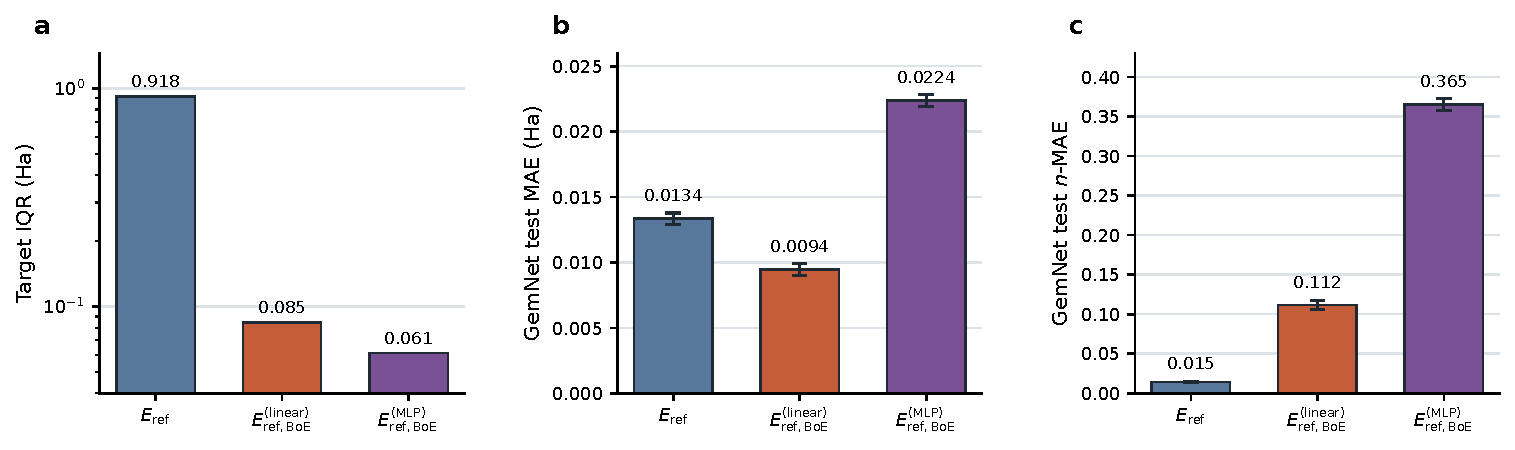
\includegraphics[width=\linewidth]{fig01_reference_correction}
  \caption{\textbf{Target scale and GemNet accuracy after BoE correction.} \textbf{a,} Test-set IQR for \(E_{\rm ref}\) and its linear- and MLP-BoE residuals. \textbf{b,} Mean GemNet test MAE. \textbf{c,} Normalized MAE, \(n\text{-MAE}_{\rm test}=\operatorname{MAE}_{\rm test}/\operatorname{IQR}_{\rm test}(y)\). Error bars show sample standard deviations across three seeds.}
  \label{fig:reference-correction}
\end{figure}

In addition to its conventional role in improving optimization and training stability, linear BoE correction reduces the mean tmQM test MAE by a factor of \(1.41\) (Fig.~\ref{fig:reference-correction}b). BoE correction is therefore a successful form of delta learning. However, this improvement could arise either from target shrinkage or from a transformation that makes the residual better aligned with GemNet's inductive bias and, consequently, easier to learn relative to its scale.

To distinguish these effects, we use the normalized MAE, \(n\text{-MAE}_{\rm test}=\operatorname{MAE}_{\rm test}/\operatorname{IQR}_{\rm test}(y)\), where the interquartile range (IQR) measures the central scale of the test target. The \(n\)-MAE provides an empirical, model-dependent measure of learning difficulty after accounting for target scale. Under a pure rescaling, MAE and IQR change by the same factor, leaving \(n\)-MAE unchanged. An algebraic rescaling control confirms this invariance (SI Note~2). An increase in \(n\)-MAE after a target transformation therefore indicates that the transformed target is harder for the same model to learn relative to its own scale, whereas a decrease indicates improved model-relative learnability.

For linear BoE correction, the \(n\)-MAE of \(E_{\rm ref,BoE}\) is \(7.7\)-fold larger than that of \(E_{\rm ref}\) (Fig.~\ref{fig:reference-correction}c), while the target IQR decreases by a factor of \(10.9\) (Fig.~\ref{fig:reference-correction}a). The reduction in absolute MAE therefore does not result from improved model-relative learnability. Instead, the substantial target shrinkage outweighs the increase in normalized learning difficulty.

The linear BoE result demonstrated that substantial target shrinkage can improve absolute performance despite reducing normalized learnability. To test whether further target shrinkage continues to improve downstream performance, we replace linear BoE with a nonlinear MLP fitted to the same elemental-count inputs. This control increases baseline flexibility while holding its input information fixed. The MLP residual is \(1.38\)-fold smaller by IQR, but its \(n\)-MAE is \(3.27\)-fold larger, resulting in a \(2.37\)-fold increase in absolute MAE (Fig.~\ref{fig:reference-correction}). SchNet shows the same trend (SI Section~1). This result rejects the assumption that progressively removing more target variation necessarily produces progressively better residual learning.

These results establish the central problem addressed in this work: baseline accuracy and its accompanying residual scale reduction alone cannot predetermine the success of a target transformation. While the normalized error assesses scale-independent learnability of the target, it remains a post-hoc metric only available after training. A practical target-design strategy therefore requires a pre-training measure that estimates how a baseline transformation changes the normalized learnability of its residual.

\subsection{Pre-training roughness quantifies model-relative learnability}
\label{sec:pretraining-roughness}

To evaluate whether a baseline residual will be learnable downstream, we measure its smoothness relative to structural information accessible to the target neural network. However, because the trained internal representations of message-passing networks such as SchNet and GemNet are learned during optimization, they are unavailable \textit{a priori}. We address this by constructing fixed, explicit geometric feature spaces, termed \textbf{representation proxies}, that approximate the geometric information available to each architecture:

\begin{itemize}
  \item \textbf{Pair-Radial Expansion (PRE):} a two-body feature space that expands element-resolved pairwise interatomic distances, \(r_{ij}\), using Gaussian radial basis functions up to a local spatial cutoff. By capturing distance distributions without explicit angular information, PRE serves as a representation proxy for pairwise message-passing architectures such as SchNet.
  \item \textbf{PRE with angular terms (PRE+A):} an extended three-body feature space that augments PRE with central-element-resolved triplet angle distributions, \(\theta_{ijk}\). By capturing angular geometry in addition to pairwise distances, PRE+A serves as a proxy for directional, triplet-based architectures such as GemNet.
\end{itemize}

Detailed descriptor formulations, radial basis dimensions, and hyperparameter choices are provided in Methods (Sections~\ref{sec:methods-baselines} and~\ref{sec:methods-roughness-diagnostics}) and SI Methods.

By mapping molecules into these proxy feature spaces, we can evaluate target variation before model optimization. We construct a \(k\)-nearest-neighbour graph connecting test molecules with similar standardized descriptor vectors. Edge weights, \(w_{ij}\), encode feature-space similarity through a locally scaled Gaussian kernel of cosine distance:
\begin{equation}
  w_{ij}=\exp\!\left(-\frac{d_{ij}^{2}}{\sigma_i\sigma_j}\right),
  \label{eq:dirichlet-edge-weight}
\end{equation}
Here, \(d_{ij}\) is the cosine distance between standardized descriptor vectors for molecules \(i\) and \(j\), and \(\sigma_i\) is a local distance scale, defined as the distance from molecule \(i\) to its \(k\)-th nearest neighbour.

Using these edge weights, we quantify target variation through the IQR-normalized graph Dirichlet roughness, \(D_{\rm IQR}\) \cite{belkin2006manifold}:
\begin{equation}
  D_{\rm IQR}(y)=\frac{1}{\sum_{\{i,j\}\in\mathcal E}w_{ij}}
  \sum_{\{i,j\}\in\mathcal E}
  w_{ij}\frac{(y_i-y_j)^2}{\operatorname{IQR}_{\rm test}(y)^2}.
  \label{eq:dirichlet-roughness}
\end{equation}
Here, \(\mathcal E\) is the set of unique undirected graph edges. For targets with nonzero IQR, this formulation normalizes local squared target differences by the squared central target spread, making \(D_{\rm IQR}\) invariant to nonzero uniform target rescaling. A lower value indicates that molecules with similar proxy descriptors have similar target labels relative to this central spread. This provides an architecture-informed, pre-training diagnostic for assessing residual learnability without first training a downstream GNN; its predictive value is tested in the following comparisons.

Applying this normalized roughness metric to the composition-corrected energy targets, we find that \(D_{\rm IQR}\) increases from \(0.548\) for \(E_{\rm ref}\) to \(1.127\) for linear-BoE and \(1.658\) for MLP-BoE. This ordering matches the post-training \(n\)-MAE ordering observed in Figure~\ref{fig:reference-correction}. The MLP-BoE residual is similarly rougher than linear-BoE in the SchNet-aligned PRE space (\(1.709\) versus \(1.152\); SI Note~6).

In the following sections, we further test whether \(D_{\rm IQR}\) can serve as a reliable qualitative ordering proxy for target roughness and whether that roughness describes the intrinsic learnability assessed post-training using \(n\)-MAE.

\subsection{Residual roughness guides target design beyond baseline accuracy}
\label{sec:residual-design}

To test whether \(D_{\rm IQR}\) reliably predicts downstream learnability, we systematically evaluated how different baseline physical approximations alter residual scale, roughness, and deep model performance. Our goal is to construct simple, computationally inexpensive baseline models that predict the atom- and composition-referenced DFT energy, \(E_{\rm ref,BoE}^{\rm DFT}\). Subtraction of these predictions, \(\widehat{E}_b\), yields the transformed residual target, \(\Delta^b\), on which the downstream GNN models are trained.

We compare three descriptor-based baselines, BoB, PRE, and PRE+A, that capture progressively richer structural information. Alongside these, we evaluate xTB as our primary semiempirical comparison and DFTB as a supporting control. Table~\ref{tab:baseline-models} summarizes the five approaches:

\begin{enumerate}
  \item \textbf{Bag-of-Bonds (BoB):} a simple global descriptor tracking RDKit-derived typed-bond counts to capture basic compositional and functional-group variation, rather than the Coulomb-matrix entries used in the conventional BoB descriptor.
  \item \textbf{Pair-Radial Expansion (PRE):} repurposing the pairwise geometric representation introduced in Section~\ref{sec:pretraining-roughness} as an explicit input descriptor to capture local two-body geometry.
  \item \textbf{PRE with angular terms (PRE+A):} repurposing the three-body geometric representation from Section~\ref{sec:pretraining-roughness} as an input descriptor to capture local pairwise and angular geometry.
  \item \textbf{Extended tight-binding (xTB):} a semiempirical quantum-mechanical baseline providing molecule-wide electronic-structure information beyond the local geometric cutoffs of the descriptors.
  \item \textbf{Density functional tight-binding (DFTB\(\dagger\)):} a second semiempirical quantum-mechanical baseline used to test whether the trends observed with xTB extend to another electronic-structure method.
\end{enumerate}

\begin{table}[H]
  \centering
  \caption{\textbf{Baseline models used for target transformation.}}
  \label{tab:baseline-models}
  \small
  \setlength{\tabcolsep}{4pt}
  \renewcommand{\arraystretch}{1.2}
  \begin{tabular}{@{}>{\raggedright\arraybackslash}p{0.12\linewidth}>{\raggedright\arraybackslash}p{0.25\linewidth}>{\raggedright\arraybackslash}p{0.19\linewidth}>{\raggedright\arraybackslash}p{0.38\linewidth}@{}}
    \toprule
    Baseline model & Input features & Fitting approach & Physical/representation target \\
    \midrule
    BoB & Typed-bond counts (\mbox{RDKit}) & Linear / MLP & Compositional and functional-group variation \\
    PRE & Pairwise distances (\(r_{ij}\)) & Linear / MLP & Local two-body geometry (SchNet proxy) \\
    PRE+A & Distances and angles (\(r_{ij},\theta_{ijk}\)) & Linear / MLP & Local three-body geometry (GemNet proxy) \\
    xTB & Atomic identities and molecular coordinates & Semiempirical QM & Non-local electronic and higher-order interactions \\
    DFTB\(\dagger\) & Atomic identities and molecular coordinates & Semiempirical QM & Molecule-wide electronic structure; supporting comparison with xTB \\
    \bottomrule
  \end{tabular}
\end{table}

For each descriptor (BoB, PRE, and PRE+A), we fit both a linear regression model and a nonlinear multilayer perceptron (MLP); the MLPs share a unified hidden architecture (Methods). This dual-fitting strategy enables two controlled evaluations: varying the input descriptor under a fixed MLP architecture assesses how baseline information content alters residual structure, while comparing linear and MLP fits within the same descriptor family isolates the effect of baseline fitting capacity. For each supervised baseline \(b\), the target residual is defined as:

\begin{equation}
\Delta^b=E_{\rm ref,BoE}^{\rm DFT}-\widehat{E}_b,
\label{eq:descriptor-delta}
\end{equation}

In parallel, we evaluate xTB to provide a physics-based baseline that accounts for non-local electronic interactions \cite{bannwarth2019gfn2xtb}. Its residual, \(\Delta^{\rm xTB}\), is computed after applying the same atom- and composition-referencing protocol:

\begin{equation}
\Delta^{\rm xTB}
=E_{\rm ref,BoE}^{\rm DFT}-E_{\rm ref,BoE}^{\rm xTB}.
\label{eq:xtb-delta}
\end{equation}

The DFTB residual is constructed in the same way, using the atom- and composition-referenced DFTB energy \cite{elstner1998sccdftb,hourahine2020dftbplus}. DFTB calculations failed for 362 neutral tmQM molecules, so this control uses the successful-calculation subset and one GNN seed per architecture. DFTB\(\dagger\) is shown in the main figures for comparison but excluded from pooled correlations and regression fits. Matched-subset comparisons and calculation details are provided in SI Note~8.

Comparing MLP baselines across descriptor families reveals a clear trade-off between target accuracy and learnability. Progressing from BoB to PRE and PRE+A progressively increases baseline accuracy and reduces residual magnitude (Fig.~\ref{fig:residual-design}a,c). Judged strictly by baseline accuracy or residual scale, PRE+A would appear to offer the optimal \(\Delta\)-learning target. However, our roughness analysis yields a different conclusion. Although these baselines reduce target IQR by factors of \(3.3\), \(4.2\), and \(4.7\), respectively, they increase representation-space target roughness (\(D_{\rm IQR}\)) by factors of \(3.3\), \(9.5\), and \(7.6\) within GemNet-aligned PRE+A space (Fig.~\ref{fig:residual-design}b). Consequently, these smaller residuals remain rougher, and none improves GemNet test MAE over direct training on \(E_{\rm ref,BoE}\).

\begin{figure}[t]
  \centering
  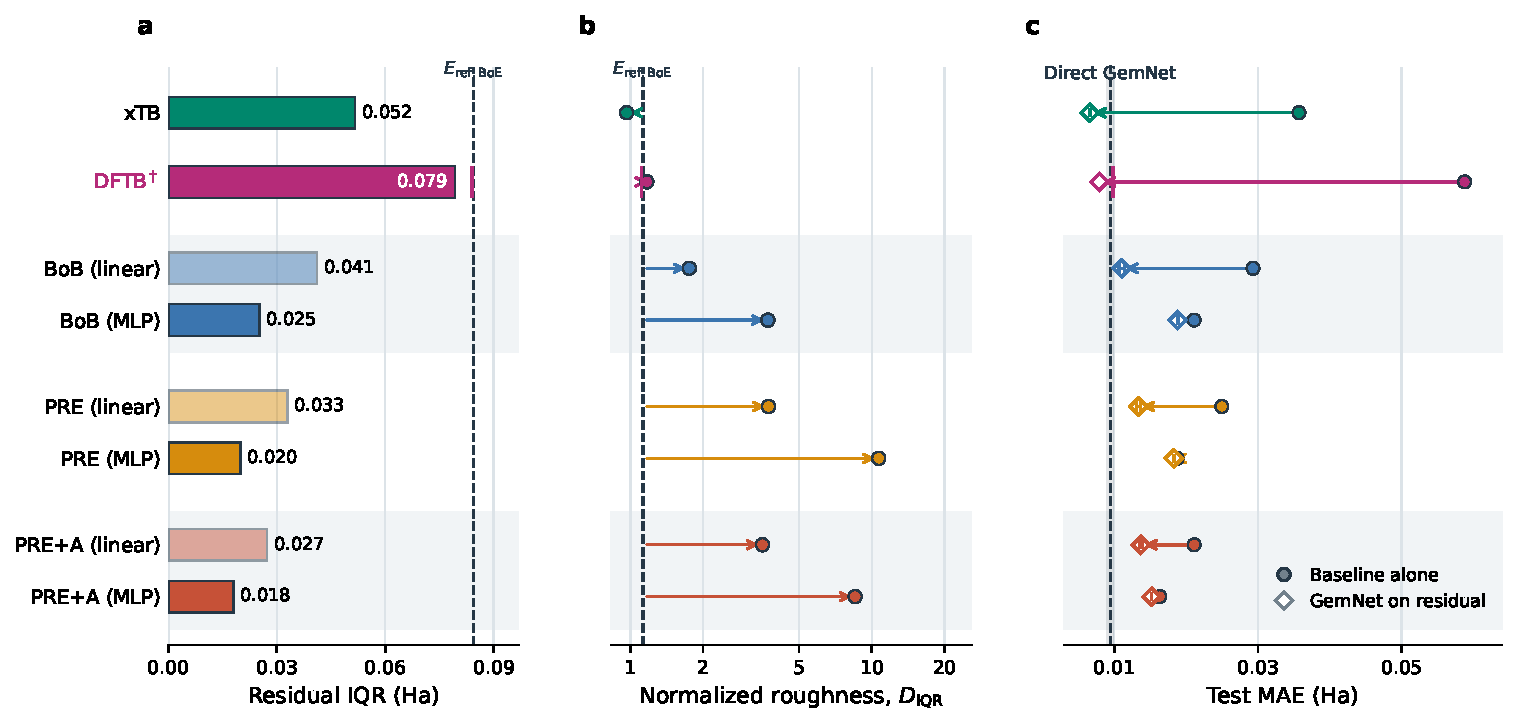
\includegraphics[width=\linewidth]{fig02_residual_design}
  \caption{\textbf{Baseline accuracy, residual roughness, and GemNet test performance.} \textbf{a,} Test residual IQR. \textbf{b,} Normalized roughness on the test PRE+A graph (log scale). \textbf{c,} Baseline-only test MAE (filled circles) and GemNet residual test MAE (open diamonds). Dashed lines mark the DFT-BoE parent or direct-GemNet reference; arrows show the corresponding changes. Main GNN results are three-seed means; error bars and shading show sample SD. Magenta DFTB\(^\dagger\) is a single-seed, valid-subset control, excluded from pooled analyses. Short magenta ticks mark its matched-subset parent references (SI Note~8).}
  \label{fig:residual-design}
\end{figure}

This degradation in learnability persists even when baseline input features remain fixed. Comparing linear and MLP fits within each descriptor family shows that increasing baseline expressivity consistently yields smaller yet rougher residuals, degrading GemNet test performance (Fig.~\ref{fig:residual-design}). For instance, transitioning from a linear to an MLP fit on BoB features reduces residual IQR by an additional factor of \(1.6\), yet GemNet test MAE increases \(1.7\)-fold. Thus, stripping away additional target variance without considering representation alignment can actively impede model generalization.

The poorer test performance on these rough residuals persists after normalization by test target IQR. For GemNet, the MLP-PRE residual has a normalized test error \(7.2\)-fold higher than the xTB residual. SchNet exhibits a similar discrepancy, with a \(4.9\)-fold difference (SI Note~6). Thus, even after accounting for target scale, the smaller MLP-PRE residual remains harder to predict on unseen structures.

In contrast, xTB leaves a larger residual than the BoB, PRE, and PRE+A baselines, yet GNNs trained on this residual achieve lower test errors. Among the primary baselines in Figure~\ref{fig:residual-design}, xTB is the only one that lowers both normalized roughness and GemNet test MAE: \(D_{\rm IQR}\) falls from \(1.127\) to \(0.964\), while mean test MAE falls from \(0.00945\) to \(0.00660\)~Ha. xTB therefore provides our primary evidence that smaller residuals are not necessarily easier for a GNN to learn.

DFTB provides a contrasting control on its valid subset: its residual is also relatively large, and has slightly higher roughness than the matched DFT parent in both PRE and PRE+A spaces. In PRE+A space, \(D_{\rm IQR}\) rises from \(1.113\) to \(1.169\), while the matched seed-101 GemNet test MAE falls from \(0.00979\) to \(0.00794\)~Ha (SI Note~8). DFTB remains a separate semiempirical control, not part of the pooled analysis. These results do not suggest that larger residuals are inherently better. Rather, they show that an effective baseline must leave a residual that the downstream model can learn, not simply one with a smaller magnitude.

\subsection{Model-relative target roughness predicts scale-normalized learnability}
\label{sec:roughness-predicts}

Can target roughness measured prior to training identify which targets a GNN will learn more accurately? We address this by comparing representation-space roughness (\(D_{\rm IQR}\)) with scale-normalized test error (\(n\text{-MAE}=\operatorname{MAE}_{\rm test}/\operatorname{IQR}_{\rm test}(y)\)). Graph-based smoothness provides a geometric framework for relating labels to neighbouring representations.\cite{belkin2006manifold} Normalized error assesses how accurately a model predicts each target relative to that target's intrinsic spread, enabling comparisons across energy targets with widely different scales.

We evaluated all 13 primary targets: atom-referenced DFT energy, linear and MLP Bag-of-Elements (BoE) residuals, referenced xTB energies and their DFT residuals, and linear and MLP residuals derived from BoB, PRE, and PRE+A representations. Because the proxy feature graph remains fixed across targets for a given architecture, differences in \(D_{\rm IQR}\) reflect how target values vary relative to their spread between neighbouring molecules, rather than changes in graph connectivity.

\begin{figure}[H]
  \centering
  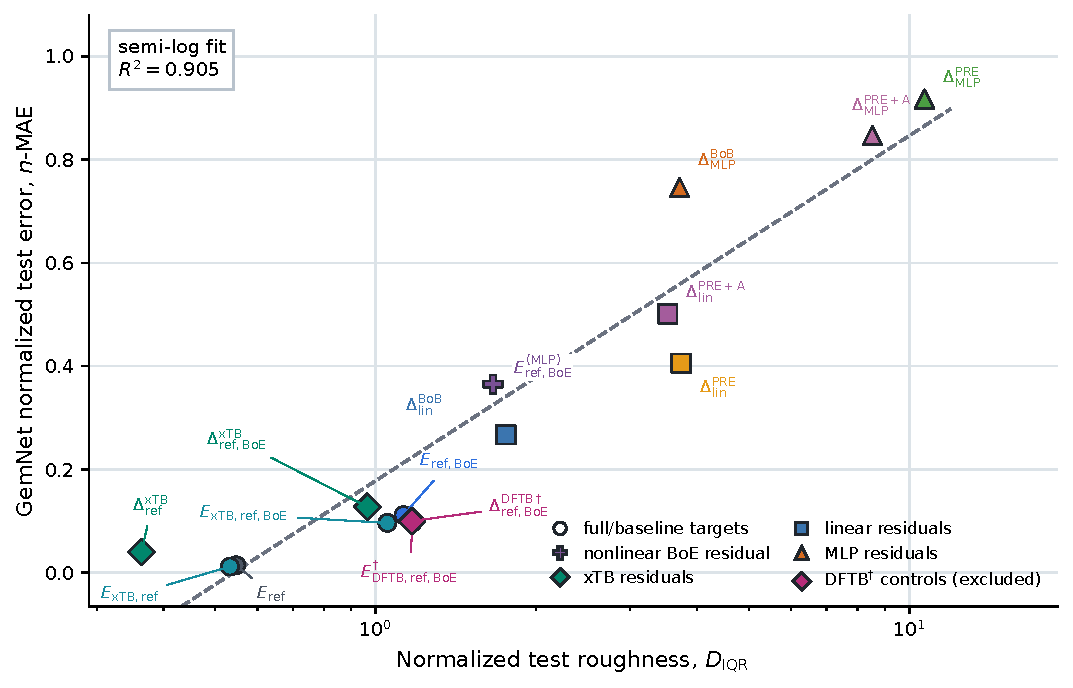
\includegraphics[width=0.90\linewidth]{fig04_roughness_nmae}
  \caption{\textbf{Model-relative roughness and normalized GemNet test error.} Mean GemNet test \(n\)-MAE, defined as \(\operatorname{MAE}_{\rm test}/\operatorname{IQR}_{\rm test}(y)\), is plotted against test \(D_{\rm IQR}\) for 13 primary targets. Roughness is measured on the standardized test PRE+A graph, and the horizontal axis is logarithmic. Marker shapes identify the target classes shown in the legend. Points show means across three GNN seeds. The dashed line is the semi-log regression over the 13 primary target means (\(R^2=0.905\)). Magenta DFTB\(^\dagger\) points are single-seed, valid-subset controls, excluded from the regression and correlations.}
  \label{fig:roughness-nmae}
\end{figure}

Across these primary targets, GemNet's normalized test error increases approximately linearly with \(\log D_{\rm IQR}\), yielding \(R^2=0.905\) in PRE+A space (Fig.~\ref{fig:roughness-nmae}). SchNet exhibits a corresponding association in PRE space (\(R^2=0.946\); SI Note~6). Practically, targets that vary more sharply between structurally similar molecules tend to be harder for downstream GNNs to learn relative to their spread. Leave-one-target-out sensitivity checks show that this trend is not driven by any single target, maintaining \(R^2\in[0.872,0.927]\) for GemNet and \(R^2\in[0.927,0.965]\) for SchNet (SI Note~7). These ranges describe refitted associations, not cross-validated prediction scores.

Because \(D_{\rm IQR}\) and \(n\)-MAE share target IQR as a scaling factor, their correlation may partly reflect shared-denominator normalization.\cite{pearson1897spurious} We conducted sensitivity controls to assess the contribution of molecular-neighbourhood alignment beyond this coupling. Removing IQR normalization from both axes reduces \(R^2\) to 0.019 for GemNet and 0.067 for SchNet, showing that the strong normalized association does not extend to the relationship between log raw roughness and absolute test error (SI Note~7).

To assess the contribution of label alignment with molecular graph geometry, we performed 5,000 joint-label permutations (SI Note~7). Shuffling target values across molecules preserves target distributions and IQRs while severing their connection to chemical structure; graphs and GNN test errors remain fixed. Although target distributions and normalization sustain a high shuffled correlation (median \(R^2=0.862\) for GemNet and 0.855 for SchNet), the observed positive correlation exceeds every shuffled result for both models (one-sided \(p\approx0.00020\), using the plus-one correction;\cite{phipson2010permutation} SI Note~7). Furthermore, among all three target pairs whose IQRs differed by at most 10\%, the smoother target also had the lower mean normalized test error for both SchNet and GemNet (SI Note~7).

Together, these results support architecture-aligned target roughness (\(D_{\rm IQR}\)) as a scale-invariant candidate pre-training diagnostic of relative target learnability. Molecular-neighbourhood alignment contributes information beyond the shuffled target-distribution baseline, although normalization contributes substantially to the observed association. These retrospective results do not establish a causal mechanism or guarantee predictive performance for new target families.

\subsection{Target design controls out-of-domain transfer}
\label{sec:ood-transfer}

To evaluate whether favourable target design enhances transferability beyond the training distribution, we tested model predictions on the QM9 dataset \cite{ramakrishnan2014quantum}. While QM9 shares elements with tmQM, it shifts the chemical domain from transition-metal complexes to small organic molecules, altering molecular size, bonding motifs, and coordination environments. To isolate this chemical domain shift from discrepancies in electronic-structure fidelity, QM9 DFT reference energies were recomputed at the identical level of theory used for tmQM, with transformed targets generated using frozen, train-only baseline parameters (SI Methods).

Evaluating out-of-domain (OOD) performance across distinct chemical families can introduce systematic dataset-level energy offsets due to divergent stoichiometry and size distributions. Because raw OOD MAE combines these global offsets with molecule-to-molecule errors, we assessed trend preservation using two complementary metrics: Kendall rank correlation (\(\tau\)), which quantifies energetic ordering, and mean-shifted MAE, which measures residual scatter after removing a single dataset-wide offset (SI Note~5). This offset is estimated from the QM9 reference labels, rendering mean-shifted MAE an oracle diagnostic rather than an independently calibrated prediction score. All reconstructed routes were mapped back onto the parent DFT-BoE energy target prior to comparison.

\begin{figure}[H]
  \centering
  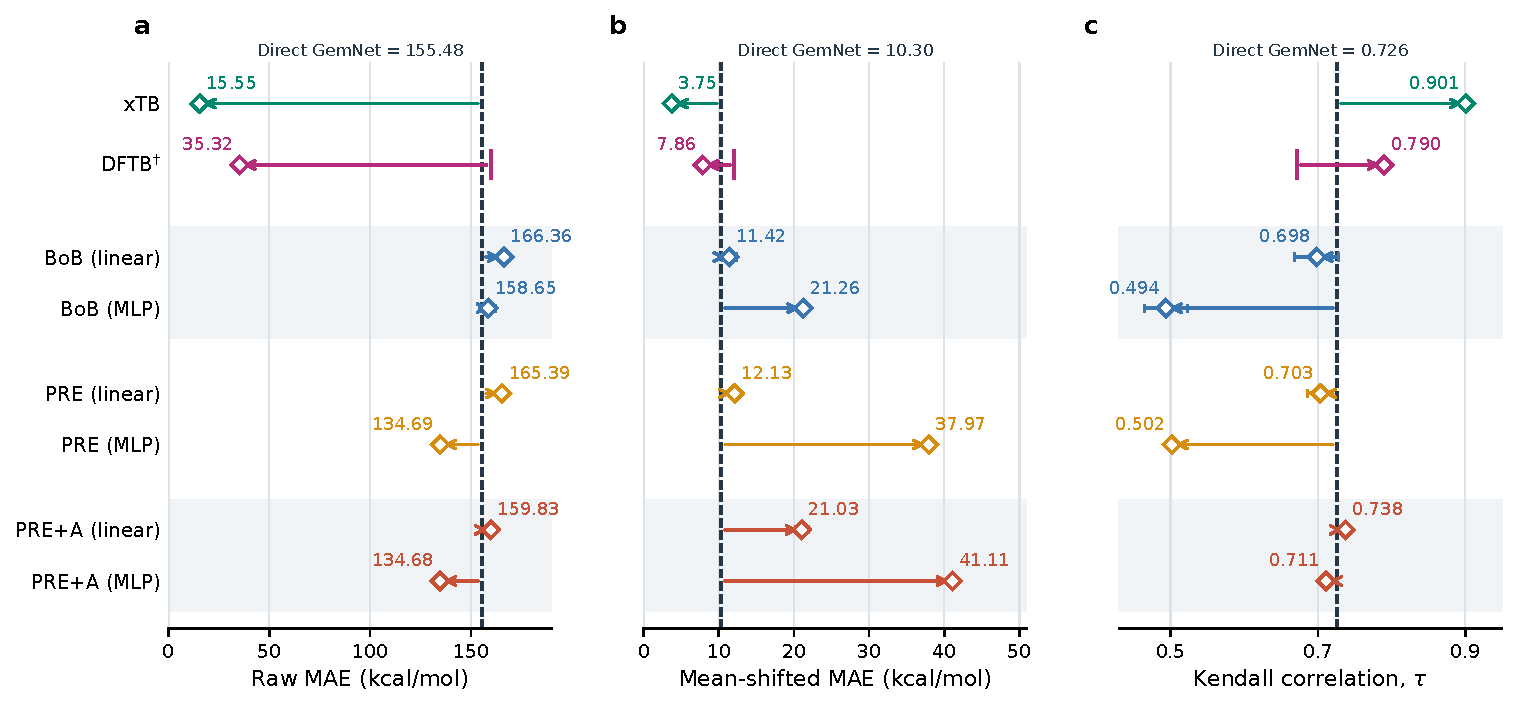
\includegraphics[width=\linewidth]{fig03_qm9_transfer}
  \caption{\textbf{Out-of-domain GemNet transfer from tmQM to QM9.} \textbf{a,} Raw MAE. \textbf{b,} Mean-shifted MAE using one offset estimated from QM9 labels. \textbf{c,} Kendall correlation. Diamonds show baseline-plus-GemNet predictions against \(E_{\rm ref,BoE}\); dashed lines mark direct GemNet. Primary results are three-seed means with sample-SD bars on 128,988 common molecules. Magenta DFTB\(^\dagger\) is a seed-101 control on 128,978 valid molecules; its short reference ticks and arrows use direct seed 101 on the same subset (SI Notes~5 and 8).}
  \label{fig:qm9-transfer}
\end{figure}

Among all primary GemNet routes evaluated on QM9, the composition-referenced xTB residual achieved the best mean transfer performance across the three reported metrics (Fig.~\ref{fig:qm9-transfer}). Learning on the xTB residual reduced mean-shifted MAE from \(0.01641\)~Ha for direct GemNet to \(0.00598\)~Ha while increasing Kendall \(\tau\) from \(0.726\) to \(0.901\) (Fig.~\ref{fig:qm9-transfer}b,c). It also yielded the lowest raw MAE, reducing error from \(0.2478\) to \(0.0248\)~Ha (Fig.~\ref{fig:qm9-transfer}a), showing that its transfer advantage does not rely on mean-shift offset calibration. In contrast, no local descriptor baseline improved upon direct GemNet on both trend metrics; linear PRE+A slightly increased mean Kendall correlation (\(\tau=0.738\)) but increased mean-shifted MAE to \(0.03351\)~Ha (Fig.~\ref{fig:qm9-transfer}b,c). Furthermore, GemNet preserved the ordering of the predicted xTB residual itself (\(\tau=0.789\) on the common QM9 cohort), supporting transfer of the learned residual correction rather than only the reconstructed energy ranking (SI Note~5). SchNet exhibited parallel improvements on the xTB residual, reducing mean-shifted MAE from \(0.01563\) to \(0.00665\)~Ha and increasing Kendall \(\tau\) from \(0.746\) to \(0.895\) (SI Note~5).

Semiempirical density-functional tight-binding (DFTB\(^\dagger\)) provided supporting evidence on its valid subset, reducing raw MAE from \(0.2547\) to \(0.0563\)~Ha, reducing mean-shifted MAE from \(0.01917\) to \(0.01253\)~Ha, and increasing Kendall \(\tau\) from \(0.671\) to \(0.790\) relative to matched-subset direct GemNet (SI Notes~5 and 8). This seed-101 control uses a different training subset and does not provide a three-seed uncertainty estimate.

These results motivate the principle of \textbf{baseline complementarity} in physical target design. Baselines constructed from local geometric descriptors share information with message-passing GNNs and may remove smooth variations that message-passing layers naturally learn while leaving behind residuals that are rough relative to their scale. In contrast, semiempirical quantum methods supply molecule-wide electronic-structure priors---including interactions beyond standard spatial cutoffs---that may complement downstream neural architectures. Tu and Rowley demonstrated such complementarity for long-range interactions, showing that a DFTB3 baseline supplies intermolecular interactions beyond a local neural network's cutoff and improves transferability over direct learning \cite{tu2026transferable}. While target scale and representation smoothness provide complementary diagnostics rather than strict guarantees for transfer, combining semiempirical physical baselines with architecture-aligned GNNs improves out-of-domain generalization in the present comparisons; the specific physical mechanism remains unresolved.

\section{Discussion}
\label{sec:discussion}

In scientific machine learning, $\Delta$-learning rests on a compelling intuition: rather than predicting a high-fidelity quantum-mechanical energy from scratch, a GNN should learn the correction to a cheap approximate baseline. Because the baseline captures much of the variation in the target, the resulting residual is smaller and presumed easier to learn. Yet, as our findings demonstrate, this intuition does not always hold. Aggressively shrinking total target scale does not guarantee downstream learnability, explaining why $\Delta$-learning has often relied on trial-and-error heuristics rather than design principles.

Our results resolve this inconsistency by reframing $\Delta$-learning as a functional target transformation governed by two distinct properties: \textbf{target scale} and \textbf{scale-normalized representation smoothness}, which tracks downstream learnability as assessed by $n\text{-MAE}$. Because absolute test error is the product of target scale and normalized error, aggressive scale reduction can still yield a net accuracy gain if the shrinkage outweighs the accompanying loss in learnability—as seen with the linear Bag-of-Elements (BoE) baseline. However, pushing shrinkage even further with a nonlinear MLP-BoE baseline raises normalized error enough to outweigh the further reduction in target scale and degrades performance.

Optimal $\Delta$-learning therefore requires \textbf{baseline complementarity}: we propose prioritizing baselines that capture the specific components responsible for the model's error, rather than merely absorbing the largest share of total target spread. Local descriptor baselines (Bag-of-Bonds, PRE, and PRE+A) share geometric information with local message-passing GNNs; they strip away smooth local features the network already represents efficiently, leaving residuals that are narrower in scale yet disproportionately rough and harder to learn, resulting in poorer test performance than direct learning. Conversely, semi-empirical quantum methods (xTB and DFTB) capture electronic effects—such as charge redistribution and long-range electrostatics—that may contribute to the errors of local architectures. By absorbing the specific energy contributions that drive GNN error, complementary baselines shrink target scale while preserving or reducing scale-normalized roughness, improving test accuracy by 30–40\% and substantially enhancing energetic rank correlation across distinct chemical domains (QM9).

Because post-training evaluation requires expensive model optimization, practical target engineering requires pre-training diagnostics. To address this, we introduced the scale-normalized graph Dirichlet roughness ($D_{\rm IQR}$), which tracks target variation over architecture-aligned representation proxies without training a downstream GNN. Its strong semi-log association with normalized test error ($n\text{-MAE}$) supports $D_{\rm IQR}$ as a candidate pre-training diagnostic for screening baselines. While shared normalization contributes substantially to this association, joint-label permutation controls support an additional contribution from molecular-neighbourhood alignment.

\section{Conclusion}
\label{sec:conclusion}

This study advances $\Delta$-learning from heuristic baseline selection toward principled target design. By establishing that baseline complementarity and the balance between target shrinkage and residual smoothness govern learnability, our results position target formulation as a foundational design choice alongside network architecture, offering a clear path forward for residual learning, multi-fidelity modeling, and scientific machine learning surrogates.

\section{Methods}
\label{sec:methods}

\subsection{Datasets and targets}
\label{sec:methods-datasets-targets}

The in-domain data are the aligned neutral tmQM transition-metal complexes with \(\omega\)B97M-V/def2-SVPD energies and fixed train, validation, and test molecule identifiers \cite{balcells2020tmqm,mardirossian2016wb97mv,rappoport2010def2svpd}. The full panel contains 56,830 training, 7,104 validation, and 7,104 test molecules. The six descriptor residuals use 56,821 training and 7,103 validation molecules, while all 13 primary targets share the same 7,104 test molecules. Both architectures use identical target values and split memberships within each target. DFTB success filtering leaves 56,540 training, 7,068 validation, and 7,068 test molecules; failed calculations were not imputed. QM9 is used only for OOD evaluation; its energies were recomputed at the same level with Psi4 to avoid conflating chemical-domain shift with electronic-structure mismatch \cite{ramakrishnan2014quantum,parrish2017psi4}.

For method \(m\), molecular energies were first corrected using fixed element-wise atomic references,
\begin{equation}
  E_{\rm ref}^{m}(i)=E_{\rm raw}^{m}(i)-\sum_Z n_Z(i)\epsilon_Z^{m},
  \label{eq:atomic-reference}
\end{equation}
then corrected by a linear model of elemental counts fitted only on the tmQM training split to obtain \(E_{\rm ref,BoE}^{m}\). Atomic references are fixed external inputs, not parameters fitted to held-out molecular energies. Separate composition models are fitted for DFT, xTB, and DFTB and frozen for validation, test, and QM9 evaluation. The DFT quantity is the parent target. Delta targets subtract either a fitted descriptor baseline or the consistently referenced xTB/DFTB energy. Full target-generation, masking, and molecule-ID alignment details are in SI Methods.

\subsection{Baseline models}
\label{sec:methods-baselines}

BoE denotes elemental-count features and the standard BoE reference is linear. A composition-only control fits a nonlinear MLP to the same counts and atom-referenced DFT energy, thereby changing baseline flexibility without adding structural information. BoB denotes the study-specific RDKit-derived typed-bond-count vector, not the conventional Coulomb-matrix Bag-of-Bonds descriptor. PRE expands local element-resolved pair distances in Gaussian radial basis functions up to a spatial cutoff, and PRE+A augments PRE with central-element-resolved triplet angle distributions. BoB, PRE, and PRE+A each have linear ridge and MLP fits to the DFT-BoE parent target; all four MLP baselines share hidden widths of 512 and 128 and the same training protocol. Ridge regularization was selected by five-fold training-only cross-validation, with preprocessing refitted within each fold. Final baseline parameters and preprocessing were fitted using only the corresponding tmQM training split. The validation split was used to select each MLP checkpoint, while test labels were used only for final evaluation. Baseline fitting seed 101 defines the canonical residual targets; fitting-seed sensitivity is reported separately in SI Note~9. GFN2-xTB and DFTB are fixed semiempirical baselines \cite{bannwarth2019gfn2xtb,elstner1998sccdftb,hourahine2020dftbplus}. DFTB uses SCC-DFTB/DFTB2 with the PTBP Slater--Koster set, without third-order or dispersion corrections \cite{dftborg2025ptbp}, and only paired successful calculations; failures were not imputed. Feature dimensions, hyperparameters, and failure audits are in SI Methods and SI Note~8.

\subsection{GNN training}
\label{sec:methods-gnn-training}

GemNet-T is the primary downstream model and SchNet is the architecture control \cite{gasteiger2021gemnet,schutt2023schnetpack2}. Models were trained on energies only, without forces or periodic boundary conditions, using fixed splits, a \(6.0~\text{\AA}\) cutoff, and a common FairChem/OCP-style protocol. Every target was standardized by its own training-set mean and population standard deviation. Within each architecture, architecture settings, loss, AdamW configuration, initial learning rate, scheduler rule, batch size, and checkpoint criterion were held fixed across targets. AdamW with AMSGrad used an initial learning rate of \(5\times10^{-4}\), MSE energy loss, and an 80-epoch budget; batch sizes were 16 for SchNet and four for GemNet. ReduceLROnPlateau responded independently to each validation trajectory, with factor 0.8 and patience three, producing target-specific learning-rate schedules. Each run's best-validation checkpoint was evaluated on both the tmQM test set and QM9. All 13 primary targets use independent GNN seeds 101, 102, and 103 for both architectures; the two DFTB targets use seed 101 only for both architectures, giving 82 runs in total. Reported primary results are means of seed-level metrics, not ensemble predictions, with sample standard deviations shown where applicable. Single-seed DFTB results have no across-seed uncertainty estimate. Exact seed-level results are reported in SI Note~9. Complete configurations and training diagnostics are in SI Methods and Supplementary Table~S3.

\subsection{Roughness and transfer diagnostics}
\label{sec:methods-roughness-diagnostics}

GemNet roughness uses standardized PRE+A features and SchNet roughness uses standardized PRE features. A cosine \(k=10\) nearest-neighbour graph was built on the 7,104-molecule tmQM test cohort. Zero-variance feature channels were removed, and retained channels were divided by the graph cohort's population standard deviation without centring. This unsupervised graph preprocessing is distinct from train-only baseline preprocessing. Unique undirected union edges were assigned similarity-based weights using the locally scaled Gaussian kernel in Equation~\ref{eq:dirichlet-edge-weight}.
\begin{equation}
  w_{ij}=\exp\!\left(-\frac{d_{ij}^{2}}{\sigma_i\sigma_j}\right),
  \label{eq:dirichlet-edge-weight}
\end{equation}
Here, \(d_{ij}\) is the cosine distance between standardized descriptor vectors for molecules \(i\) and \(j\), and \(\sigma_i\) is a local distance scale, defined as the distance from molecule \(i\) to its \(k\)-th nearest neighbour.

Using these edge weights, we quantify target variation through the IQR-normalized graph Dirichlet roughness, \(D_{\rm IQR}\) \cite{belkin2006manifold}:
\begin{equation}
  D_{\rm IQR}(y)=\frac{1}{\sum_{\{i,j\}\in\mathcal E}w_{ij}}
  \sum_{\{i,j\}\in\mathcal E}
  w_{ij}\frac{(y_i-y_j)^2}{\operatorname{IQR}_{\rm test}(y)^2}.
  \label{eq:dirichlet-roughness}
\end{equation}
Here, \(\mathcal E\) is the set of unique undirected graph edges. For targets with nonzero IQR, this formulation normalizes local squared target differences by the squared central target spread, making \(D_{\rm IQR}\) invariant to nonzero uniform target rescaling.

Both \(D_{\rm IQR}\) and \(n\text{-MAE}_{\rm test}\) use the corresponding test-target IQR; graphs and weights remain fixed across primary targets within each architecture. DFTB controls use separately constructed valid-subset test graphs and are excluded from primary regressions and pooled statistics.

Semi-log regressions use unweighted ordinary least squares across the 13 primary target means, with an intercept and \(\ln D_{\rm IQR}\) as predictor. Raw-error, raw-roughness, variance-normalization, partial-correlation, and leave-one-target-out sensitivity analyses are reported in SI Note~7. The same note reports 5,000 joint test-label permutations, which preserve each target's distribution and IQR while breaking molecular-neighbourhood alignment, and comparisons of target pairs whose IQRs differ by at most 10\%. Leave-one-target-out fits are influence checks, not cross-validated prediction scores. These test-set analyses are retrospective diagnostics performed after model selection; test labels were not used to fit baselines, schedule training, or select checkpoints.

\subsection{OOD transfer evaluation}
\label{sec:methods-transfer}

tmQM-trained models were evaluated without retraining on QM9 geometries, using frozen tmQM training-only baseline parameters. Residual predictions were combined with their corresponding baselines and mapped to the common DFT-BoE parent before full-target correlation and ranking metrics were calculated. Primary parent-energy comparisons use 128,988 common QM9 molecules and three GNN seeds. The DFTB residual is shown on its 128,978-molecule intersection with this cohort, alongside a matched-subset direct seed-101 reference; this matches evaluation molecules, not training cohorts. Mean-shifted MAE removes one scalar mean-error offset estimated separately for each predictor from the evaluated QM9 reference labels and is used only as a post hoc oracle diagnostic, not an independently calibrated prediction score. Figure~\ref{fig:qm9-transfer} reports GemNet raw and mean-shifted MAEs in Ha, without IQR normalization, and Kendall correlations; exact coverage, offset magnitudes, and additional metrics are reported in SI Note~5. Detailed reconstruction and evaluation procedures are in SI Note~5.


\section*{Data and Code Availability}
The source datasets used in this work are publicly available from their original
providers: tmQM for transition-metal complexes and QM9 for small organic
molecules. The processed split identifiers, target-generation tables, baseline
fits, model-configuration files, evaluation manifests, and figure/table source
data needed to reproduce the analyses in this manuscript will be deposited in a
versioned Zenodo archive at publication. The analysis and training code will be
released in a public GitHub repository, with the corresponding Zenodo DOI cited
in the final manuscript. Large generated artifacts, including LMDB training
databases, neural-network checkpoints, prediction arrays, and learned embedding
exports, are not tracked directly in Git; when required for exact reproduction,
they will be provided through the release artifact bundle or can be regenerated
from the released scripts and the public source datasets.

\section*{Acknowledgements}
The authors acknowledge the Alliance for AI-Accelerated Materials Discovery (A3MD) for supporting the research environment, scientific exchange, and computational infrastructure that enabled this work.

\bibliographystyle{unsrt}
\bibliography{bib/references}

\end{document}
